\documentclass{standalone}
\usepackage{tikz}

\begin{document}
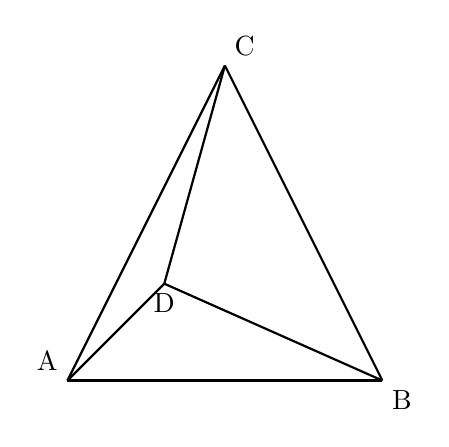
\begin{tikzpicture}[scale=2]

% Define the coordinates of the vertices
\coordinate (A) at (-1, -1, 0);
\coordinate (B) at (1, -1, 0);
\coordinate (C) at (0, 1, 0);
\coordinate (D) at (0, 0, 1);

% Draw the edges of the tetrahedron
\draw[thick] (A) -- (B);
\draw[thick] (B) -- (C);
\draw[thick] (C) -- (A);
\draw[thick] (A) -- (D);
\draw[thick] (B) -- (D);
\draw[thick] (C) -- (D);

% Label the vertices
\node[above left] at (A) {A};
\node[below right] at (B) {B};
\node[above right] at (C) {C};
\node[below] at (D) {D};

\end{tikzpicture}
\end{document}